% !TEX root = ../Thesis.tex
% !TEX spellcheck = en-US

\chapter{GNS3}
\label{ch:gns3}

GNS3, whose original name was ``Graphical Network Simulator-3,'' is a software project, comprising several distinct components and, despite the ``simulator'' in its name, \emph{as a whole}, it falls under the category of emulators (cf.~\ref{sec:emulationsimulation}): its operation runs real code accross all the layers of the stack. % TODO try to (either with a source, or speculating) relate the name with ns-3
% TODO also: cite the source for the name
% By ``as a whole,'' it is meant that, as shall be seen later, although some of its components, like the Dynamips program, are emulators in a very strict sense---i.e. its purpose is to run real machine code on a different hardware architecture (than its native one)---, it differentiates itself, on a high-level perspective, from a simulator which is a program designed to execute a mathematical model, processing modeled events as internal data-structures with a collection of preset algorithms that somehow mimic (a part of) the reality. % TODO: delete?

Note that a necessary step towards the goal of this this thesis is to systematize a technical description of the architecture and functional underpinnings of the GNS3 system.
How does it interact with the hardware and software it is running in, how much resources does it take to work with GNS3 according to the ``mode'' it is running in, etc., as that is an aspect that is yet to be further explored for, at least, the following reasons:  % TODO improve the writing how is etc written in Engilsh?
on the one hand, the consulted academic material (i.e. research papers, mostly) is very brief and omissive in regards to the design, architecture and implementation of GNS3, and so is the official website and documentation; on the other hand, many interesting details are in the ``paraofficial'' videos available via YouTube, mostly by David Bombal\footnote{\url{https://www.youtube.com/channel/UCP7WmQ_U4GB3K51Od9QvM0w}}, namely a comprehensive overview of the architecture (compared with the functionality) of GNS3 by its creator, Jeremy Grossmann, and essentially are not anywhere else, at least from authoritative sources. % TODO same as the previous "sentence". Cite the videos (how and which ones?)

% TODO add a figure (a screen shot) showing the "official" submitter of GNS3 videos (and maybe the channel and/or links from the gns3 official website)

% end of intro

% Section "GNS3's purpose and raison d'être"
\section{GNS3's purpose and \emph{raison d'être}}
\label{sec:gns3why}

The GNS3 project was co-created by Jeremy Grossmann at the University, the Ecole informatique Epitech, as part of the \emph{EPITECH Innovative Project (EIP)}\footnote{\url{https://eip.epitech.eu/2013/gns3/en/index.html}, accessed on December 2019}.
There is also a blog\footnote{\url{http://gns3.blogspot.com/2007/}, accessed on December 2019}, whose first posts date back to 2007, that announces the first ``beta'' releases of the software and gives the details about the inception of GNS3, and also lists the original developers of the project.

It may be speculated that GNS3's first ``appeal'' was supplying students of Cisco certifications with a self-study tool more powerful that anything before, one that allows for the creation of arbitrary network topologies and practice their skills with the same software stack that is used in real Cisco devices and the hosts connected to them---from the operating system, up until application--level network utilities---, without having to use the expensive official solutions for that purpose, or depending on a real, physical networking laboratory.
However, despite having kept a strong relation with training for Cisco CCNA and related certifications, the magnitude of the project, part of which comes from an inherent extensibility, has made it suitable for a myriad of use-cases.

In the industry, GNS3 naturally can come handy as a tool to prototype and test a topology for a real organization network, in the context of the practice of a network professional.
But also, in the age of the DevOps philosophy---a set of practices and methodologies/philosophies for faster delivery of applications and services---, of which \emph{infrastructure as code} is one of the culprits~\cite{awswhatisdevops}, it can be of value for software engineers to test distributed applications that depend on certain network behaviors. % TODO try to find a good list of use cases

% At the moment of the writing of this thesis, version 2.2 has recently came out\footnote{\url{https://github.com/GNS3/gns3-gui/releases/tag/v2.2.0}}.
% This version brings a lot of improvements and new features, like the new web UI or ``physical'' link state detection for QEMU nodes~\cite{releasenotesgns3v22}, and at the same time some of the ways GNS3 has been typically used are changing---such is the case of the discouragement of the usage of Dynamips and VPCS (in detriment of virtualized versions of IOS or others, or Docker containers for ``emulating'' hosts, respectively)~\cite{ytdynamipsvpcs}.


% Section "Building blocks. The programs inside GNS3"
\section{Building blocks. The programs ``inside'' GNS3}
\label{sec:gns3buildingblocks}

In an very simplified way, GNS3 is a conjunction of UI/client tools (the official GUI, the new web UI, or any custom program that ``speaks'' the documented public \acrshort{REST} API), a powerful distributed orchestrator (the \emph{controller} in the server), and a set of integrations (the so-called ``compute nodes'') with virtualization and hardware emulation tools from ``the outside'', i.e. that do not belong to the GNS3 project, like KVM, Docker, or QEMU, to provide a way to describe a topology of interconnected computing and routing nodes---that is, a computer network---, including firewalls and NAT devices, control their behavior and launch administrative tools (like \texttt{telnet} sessions). % TODO cite documentation of the REST API. Make sure we elaborate on "computes". How is so-called written - is an hyphen used?

% What follows is a description of what are those elements and what they do work internally.
% How they integrate with GNS3 or vice-versa, and also how they interact with each other, is described in~\ref{sec:gns3architecture}.

\begin{figure}
  \centering
  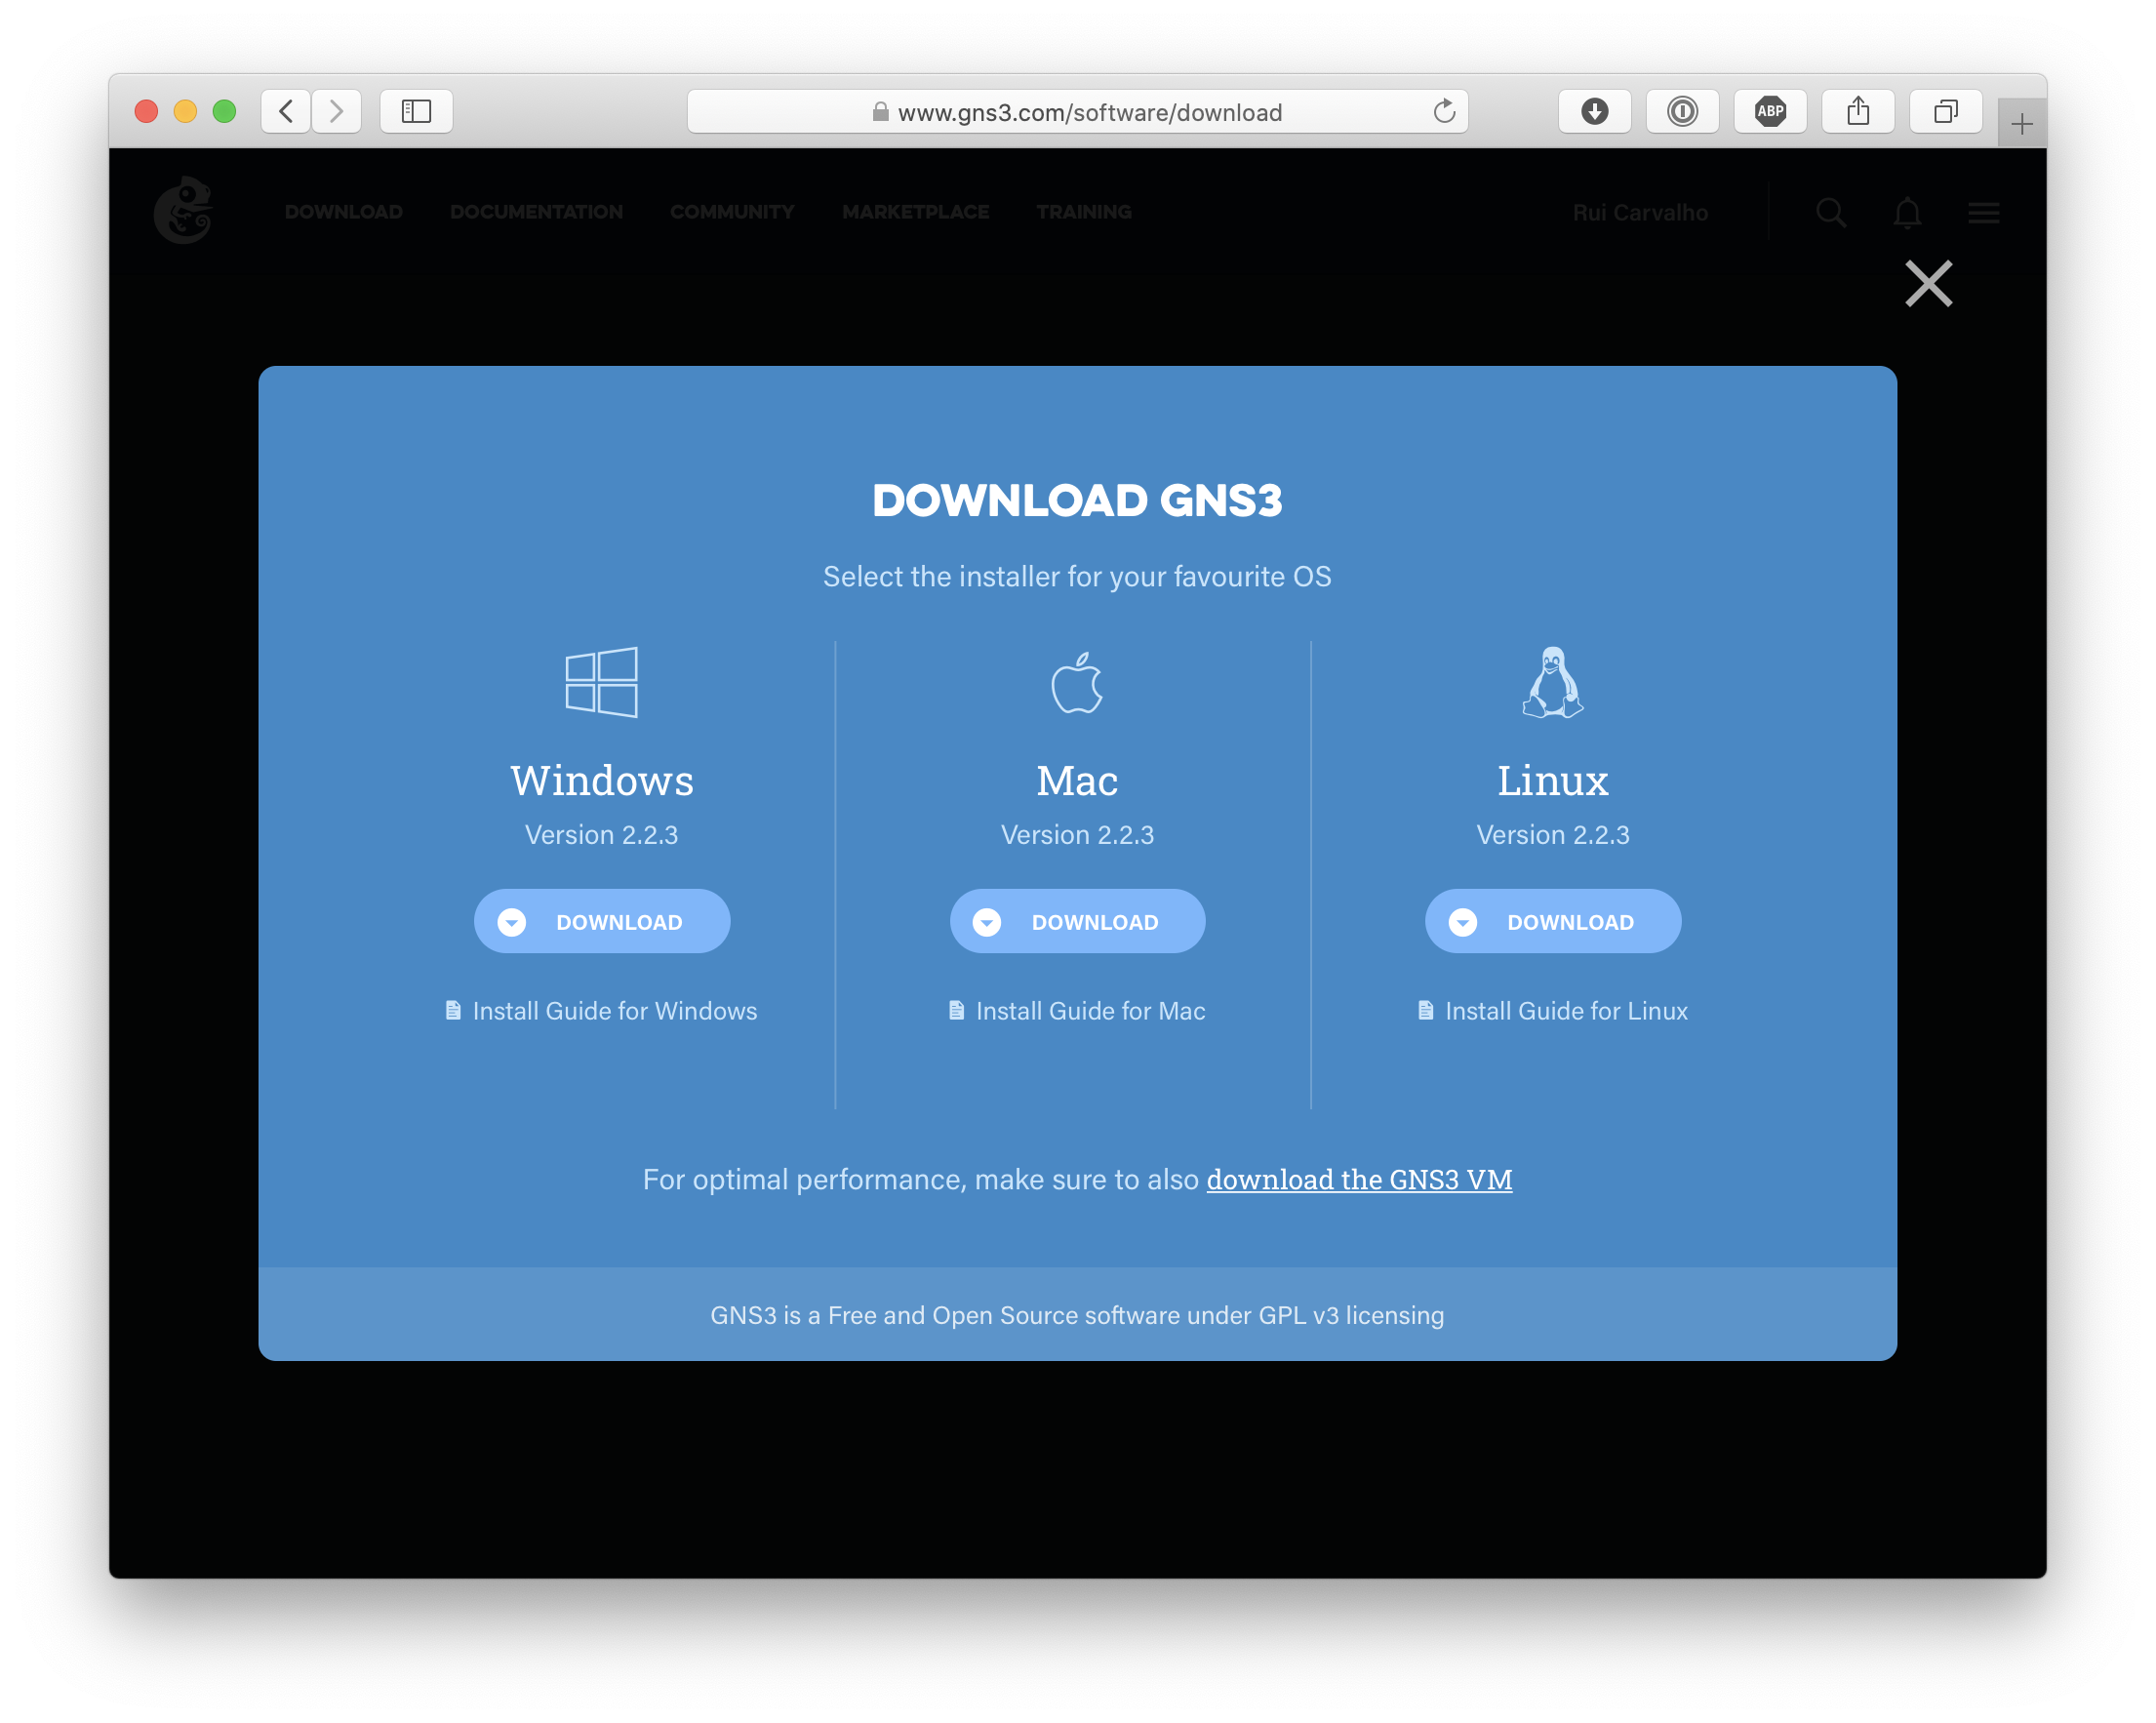
\includegraphics[width=0.8\textwidth]{download-gns3}
  \caption{The download screen on the official GNS3 website}
  \label{fig:download-gns3}
\end{figure}

When GNS3 is installed downloading one of its desktop distributions---available for Windows, macOS, and GNU/Linux, like the screen shot~\ref{fig:download-gns3} shows---, a user is installing multiple ``programs'' (or applications, whichever is the preferred denomination), implemented in disjunct codebases, and, given that they are \emph{free and open source} projects~\cite{gplv3}, hosted in GitHub, are easily accessible---and developers can enhance features and provide bugfixes.
Those are the essential building blocks of GNS3 and table~\ref{tab:gns3components} can serve a summary of what those pieces are.
It's worth noting that they are all under the GNS3 organization in GitHub\footnote{\url{https://github.com/gns3}}.

\begin{table}
  \centering
  \small
  \begin{tabulary}{0.95\textwidth}{lLL}
    \toprule
      \textbf{Part}       & \textbf{Role}                                                           & \textbf{Source code repository URL}\\
    \midrule
      GNS3 GUI            & A desktop application that runs on a graphical OS                       & \scriptsize\url{https://github.com/GNS3/gns3-gui}\\
      GNS3 server         & The main \emph{backend} implementation of GNS3. Its decision point      & \scriptsize\url{https://github.com/GNS3/gns3-server}\\
      Dynamips            & A MIPS emulator able to run legacy IOS images                           & \scriptsize\url{https://github.com/GNS3/dynamips}\\
      uBridge             & Application to bridge different user-land bridges                       & \scriptsize\url{https://github.com/GNS3/ubridge}\\
      VPCS                & A simulator for a real PC, with a few implemented commands              & \scriptsize\url{https://github.com/GNS3/vpcs}\\
    \bottomrule
  \end{tabulary}
  \caption{%
    Parts of GNS3, constituting separate and independent codebases
  }
  \label{tab:gns3components}
\end{table}


\subsection{GNS3 GUI}
\label{subsec:gns3gui}

Interaction between the end-user and GNS3 is usually---though, as will be clear, not necessarily---done in a graphical environment.
A GNS3 project, called a \emph{topology}, is constantly opened on one single window (per running instance of the application) and is graphically represented in the main section of the window.

Even though the GUI is not the authoritative source of truth for a topology (cf.~\ref{sec:gns3architecture}), it can be used as interface to all of GNS3's functionality: edit the topology itself (adding or removing nodes, changing links), performing actions on the nodes (like starting or stopping a host or router), or using helpers to launch consoles automatically connected via \texttt{telnet} or SSH.
In the section dedicated to the usage of GNS3~\ref{sec:gns3inaction}, it will be shown how this is done from a user's perspective.
Many GUI clients, on different hosts (e.g. laptops), can be editing the same topology at the same time. % TODO try to capture screenshots of this happening (use VMs)

\begin{figure}
  \centering
  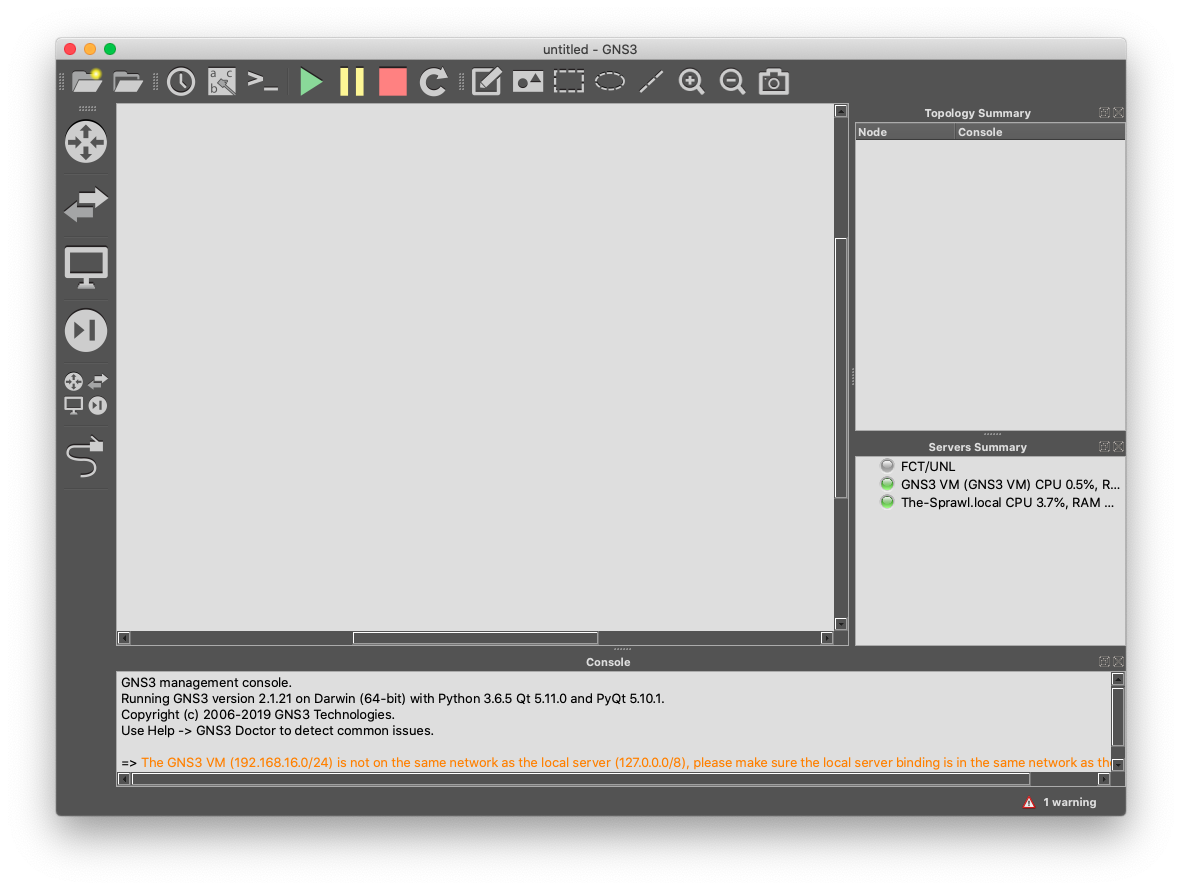
\includegraphics[width=0.8\textwidth]{gns3-empty-topology}
  \caption{An empty GNS3 topology shown in the GUI}
  \label{fig:gns3-empty-topology}
\end{figure}

\subsection{Dynamips}
\label{subsec:gns3dynamips}

The Dynamips emulator is a standalone program, written in C, that, usually, comes distributed together with the whole GNS3 package.
It is an emulator for a MIPS processor and was the original--single way to run the software of the Cisco nodes of the topologies created with GNS3.


\subsection{GNS3 server}
\label{subsec:gns3server}


\subsection{GNS3 VM}
\label{subsec:gns3vm}

% end of section gns3buildingblocks


% Section "General architecture"
\section{Architecture and building blocks}
\label{sec:gns3architecture}

A good written, comprehensive description of the GNS3 architecture and technical details is lacking.
There is a page, on the online developers-oriented documentation~\cite{gns3devarch}, which presents a very simple diagaram, that is reproduced~\footnote{Dashed strokes are added by the author of the thesis to provide extra information} on figure~\ref{fig:gns3-docs-arch}.
Even the two published books that exist on the project~\cite{gns3netsimguide,thebookofgns3} are omissive or very brief, not allowing for gaining an in-depth knowledge, necessary to understand the possible issues of performance, resource consumption, scalability, and functional limitations that GNS3 may suffer from.
Going from the simple diagram that was mentioned towards a more complete reference is one of this thesis' efforts.

To accomplish such effort, a precious resource has been the ``paraofficial'' videos available via YouTube, mostly by David Bombal, an instructor and close collaborator of the GNS3 organization, namely a comprehensive overview of the architecture (compared with the functionality) of GNS3 by its creator, Jeremy Grossmann~\cite{ytgns3arch22}, and essentially are not anywhere else, at least from authoritative sources. % TODO do nothing with \footnote{\url{https://www.youtube.com/channel/UCP7WmQ_U4GB3K51Od9QvM0w}} ?

% Figure fig:gns3-docs-arch
\begin{figure}
  \centering
  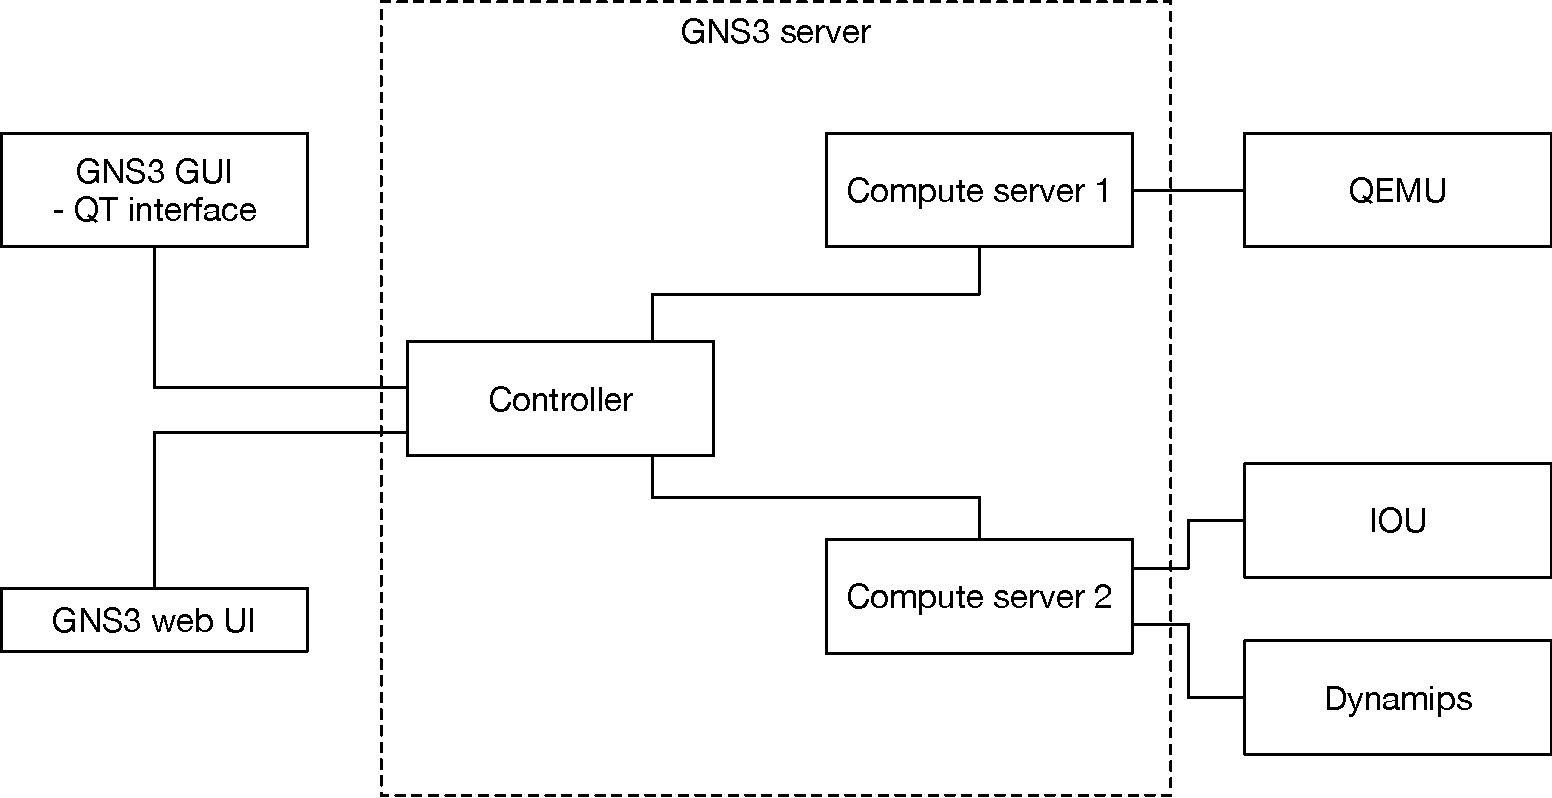
\includegraphics[width=0.8\textwidth]{gns3-docs-arch}
  \caption{The architecture of GNS3 (adapted from the official documentation)}
  \label{fig:gns3-docs-arch}
\end{figure}


\subsection{The simple client-server perspective}
\label{subsec:gns3clientserver}

GNS3 works, first and foremost, as a client-server application.
The standard installation for desktop provides all the necessary to components to fully(-ish) work on that physical machine, but the client doesn't have to be, and in many real scenarios isn't, running on the same host as the server.
However, in fact, a \textbf{topology}---the name GNS3 gives to its ``projects,'' which comprises of nodes (emulated/virtualized routers, switches, SDN-controllers, virtual PCs, interfaces for hardware network connections)---can be running in different machines, even on the ``backend'' side itself, as will be seen.

The \textbf{GNS3 server} exposes a public \acrshort{REST} \acrshort{API}, documented in~\cite{gns3devarch}, which is the way any client edits the opened topology or performs actions on the nodes contained therein, or in the GNS3 running environment.
GNS3 server, described more thoroughly afterwards, is the brains and central point of topology opened and in-execution.
It has first-hand knowledge of events that occur in the nodes, their status, their interfaces' status, and communicates with the several means existing to actually provide the \emph{emulation} for each specific node.
All of this will be analyzed and explained posteriorly.
For now, it suffices to see it as a central point, accessible by any number of clients, of a running topology.

To interact with the system, by editing a topology, or performing actions on nodes---all the items in the topology, which can be connected via links---, one or more users simultaneously can utilize a graphical client. The \textbf{GNS3 GUI}, part of a standard installation on any desktop operating system, namely macOS, a desktop Linux distribution (official repositories for Ubuntu exist), or Windows~\footnote{\url{https://gns3.com/software/download}}, is a cross-platform application developed using the Qt graphical toolkit~\cite{qttoolkit}.
They may also use a web UI (somewhat limited yet), or any tool, user-driven or automatic, programmed to send requests and receive responses according to the aforementioned REST specification.
The official clients, bundled with the GNS3 installation packages for desktop environments, GNS3 GUI and the official web UI, show an in-real-time view of the topology---e.g. the status of virtual network interfaces, or changes made by other client---thanks to WebSockets server-to-client calls~\cite{ytgns3arch22}. % TODO link WS to the glossary, when definition is available

% Figure fig:gns3-2hosts2routers-macOS
\begin{figure}
  \centering
  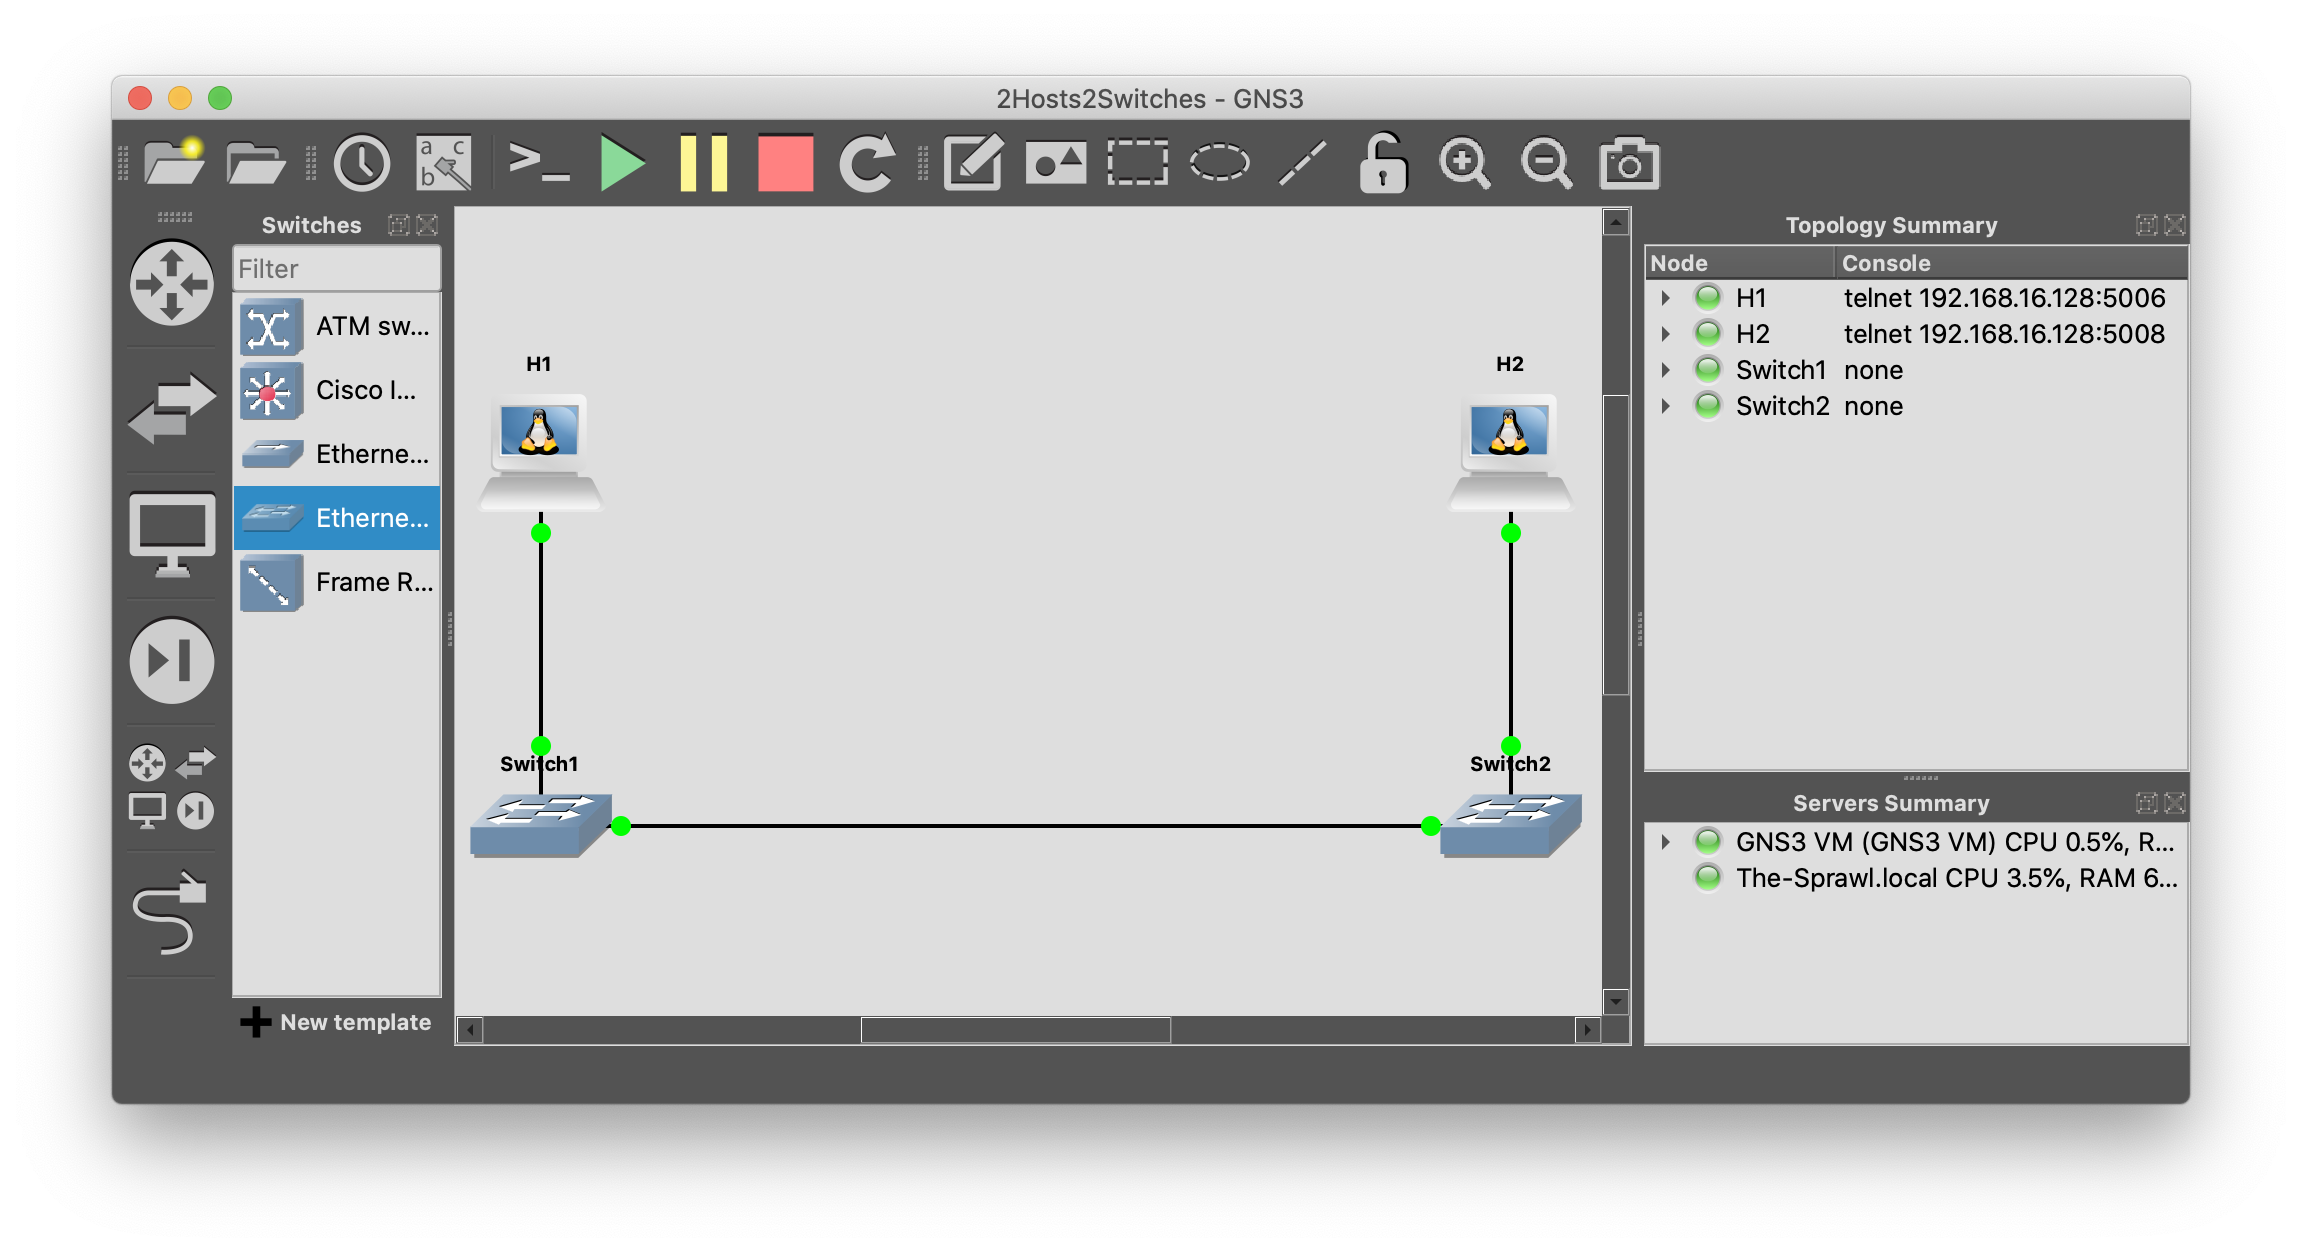
\includegraphics[width=0.8\textwidth]{gns3-2hosts2routers-macOS}
  \caption{Simple topology with only two switches and two virtual PCs as seen on the GUI in macOS}
  \label{fig:gns3-2hosts2routers-macOS}
\end{figure}


\subsection{The GNS3 server---distributed}
\label{subsec:gns3serverindetail}

The GNS3 server is a program with a code-base independent from other parts of the project.
The software package \texttt{gns3-server} can be obtained from official repositories for Linux systems to install it on servers without video interface, with users running some of the already mentioned clients in their laptops or desktop computers.
It is also possible to obtain a VMware ESXi image to directly spin-up a GNS3 server ready machine on an virtualized infrastructure.

The same program behaves as two different roles, both of which are necessary to get the GNS3 system working.

\begin{itemize}
	\item The \textbf{controller node}, or just ``controller,'' of which there can only be one instance per running topology, and is ``[its] decision point'' (Jeremy Grossmann's words); the process responsible by fulfilling the client's requests and postback real-time information to them and know the hosts where nodes may be running.
	\item The \textbf{compute node}, referred to simply as ``compute'' too, which, for one running topology, can be running $N$ times, one per each machine (physical or virtual) taking care of emulating one or more topology nodes (again: switches, routers, etc.).
	It is this separation and the ability to have multiple compute nodes that allows GNS3 to be configured in a way that can serve arbitrarily large topologies, since the cost in resources of an increasing number of ``live'' nodes can be balanced among an also increasing number of servers running a compute.
\end{itemize}

When the server is running on a single host, one \texttt{gns3-server} program instance (i.e. process) performs both roles, controller and compute.
However, when the server is distributed across one or more machines, communication between the controller and the computes on other hosts happens through a REST API.
That API is a private or internal one, unlike the one for client-server, and there isn't a programmer's manual for developing with it.
Only the (single) controller is supposed to communicate with each process acting as compute.

% end of section gns3architecture


% Section "Practical case study"
\section{Practical case study}
\label{sec:gns3practicalcasestudy}

% end of section gns3practicalcasestudy


% Section "Performance and resources considerations"
\section{Performance and resources considerations}
\label{sec:gns3performance}

% end of section gns3performance


% end of chapter
